% ============================================================
% 第3章：幂函数与多项式——变化的"速度"
% ============================================================

\chapter{幂函数与多项式——变化的"速度"}

\begin{applicationbox}
\textbf{学完本章你能做什么？}
\begin{enumerate}
  \item \textbf{学之前}：你知道 \(y = x^2\) 是抛物线，\(y = x^3\) 是三次曲线——但为什么指数不同，曲线长得不一样？
  \item \textbf{学之后}：你能一眼看出一个幂函数或多项式在 \(x\) 很大时的"走向"——向上还是向下？增长多快？
        你还会看到多项式的根如何决定它与 \(x\) 轴的交点。
  \item \textbf{日常例子}：自由落体的距离 \(s = \frac{1}{2}gt^2\) 是 \(t\) 的二次函数；\\
        物体的体积随半径的三次方增长（\(V = \frac{4}{3}\pi r^3\)）。不同指数描述不同的增长速度——这是幂函数的核心。
\end{enumerate}
\end{applicationbox}


% ============================================================
\section{从第2章来——函数的图像告诉我们什么？}
% ============================================================

第2章我们画了六种基本函数的图像，其中最关键的一个区别是\textbf{增长的"速度"}：

\begin{center}
\begin{tabular}{c|c|c}
\textbf{函数} & \textbf{当 \(x\) 很大时的行为} & \textbf{增长"等级"} \\
\hline
\(y = x\) & 直线增长 & 慢 \\
\(y = x^2\) & 抛物线增长（越来越快） & 中等 \\
\(y = x^3\) & 三次方增长（更快） & 快 \\
\end{tabular}
\end{center}

这种"增长等级"就是由\textbf{幂函数的指数}决定的。\\
指数的变化，会彻底改变曲线的形状和行为。


% ============================================================
\section{幂函数的定义}
% ============================================================

\begin{definitionbox}[幂函数]
形如
\[
y = x^n
\]
的函数称为\textbf{幂函数}（读作 mì hán shù，英文 power function），
其中 \(n\) 是\textbf{常数}（可以是整数、分数、正数、负数）。

\textbf{注意：}幂函数的特点是\textbf{底是变量 \(x\)，指数是常数 \(n\)}。
不要和指数函数 \(y = n^x\)（底是常数，指数是变量）搞混。
\end{definitionbox}

\begin{examplebox}[1——幂函数 vs 指数函数]
\begin{center}
\begin{tabular}{c|c|c}
 & \textbf{幂函数} & \textbf{指数函数} \\
\hline
形式 & \(y = x^n\) & \(y = a^x\) \\
例子 & \(y = x^2\)（底变，指数固定） & \(y = 2^x\)（底固定，指数变） \\
图像特征 & 经过 \((1,1)\) & 经过 \((0,1)\) \\
\end{tabular}
\end{center}

\textbf{记忆方法：} "幂"字下面是"幂"——底数像底座（变化），指数像屋顶（固定）。
\end{examplebox}


% ============================================================
\section{正整数幂——指数越大，增长越快}
% ============================================================

当 \(n\) 是正整数（\(n = 1, 2, 3, 4, \ldots\)）时，\(y = x^n\) 是最简单的幂函数。

\begin{examplebox}[2]
在同一坐标系中对比 \(y = x\)、\(y = x^2\)、\(y = x^3\)、\(y = x^4\)：

\begin{center}
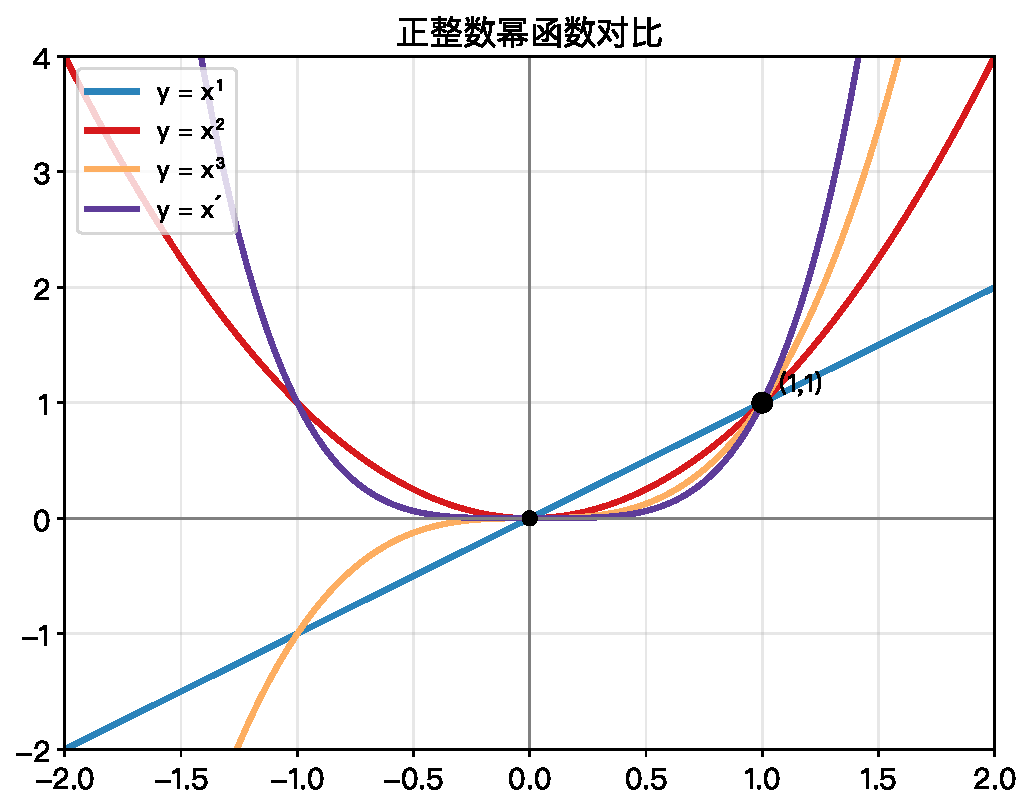
\includegraphics[width=0.6\textwidth]{figures/ch03_positive_powers.pdf}
\end{center}

\textbf{观察规律：}
\begin{enumerate}
  \item 所有图像都经过 \((0,0)\) 和 \((1,1)\)——因为 \(0^n = 0\)，\(1^n = 1\)
  \item 在 \(0 < x < 1\) 区域：指数越大，函数值越小（因为分数越乘越小）
  \item 在 \(x > 1\) 区域：指数越大，增长越快（\(x^4\) 跑得比 \(x^2\) 快得多）
  \item 偶次幂（\(n=2,4\)）的图像关于 \(y\) 轴对称，是\textbf{偶函数}
  \item 奇次幂（\(n=1,3\)）的图像关于原点对称，是\textbf{奇函数}
\end{enumerate}
\end{examplebox}

\begin{definitionbox}[奇函数与偶函数]
\begin{itemize}
  \item \textbf{偶函数}：\(f(-x) = f(x)\)，图像关于 \(y\) 轴对称（如 \(y = x^2\)）
  \item \textbf{奇函数}：\(f(-x) = -f(x)\)，图像关于原点对称（如 \(y = x^3\)）
\end{itemize}
\end{definitionbox}

\begin{examplebox}[3——奇偶性的直观理解]
\begin{itemize}
  \item \(y = x^2\)：左边和右边一样高 \(\rightarrow\) 偶函数
  \item \(y = x^3\)：左边(负)是右边(正)的倒影 \(\rightarrow\) 奇函数
  \item \(y = x\)（直线）：左边低右边高，经过原点 \(\rightarrow\) 奇函数
\end{itemize}
\end{examplebox}


% ============================================================
\section{正偶次幂与正奇次幂的"走向"}
% ============================================================

对于正整数幂，指数是奇数还是偶数，决定了函数图像\textbf{两端的走向}。

\begin{center}
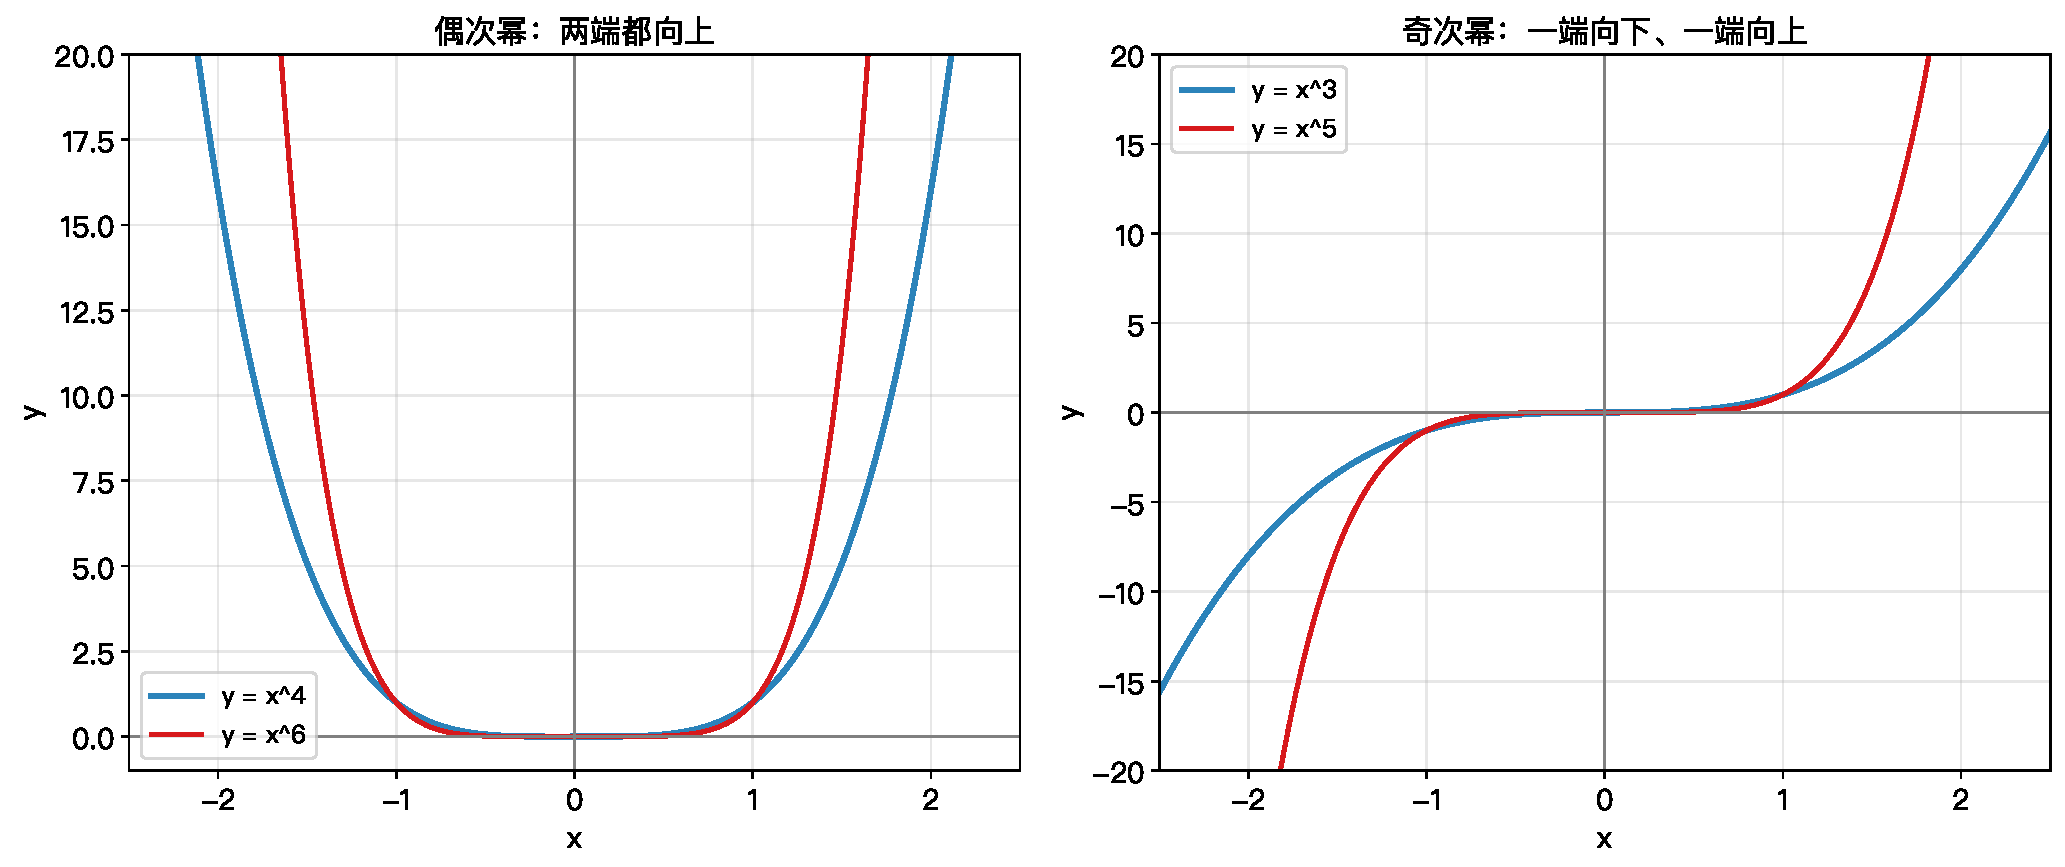
\includegraphics[width=0.75\textwidth]{figures/ch03_even_vs_odd.pdf}
\end{center}

\begin{definitionbox}[幂函数两端走向的规律]
对于 \(y = x^n\)（\(n\) 为正整数）：
\begin{center}
\begin{tabular}{c|c|c}
 & \textbf{\(x \to -\infty\)（左端）} & \textbf{\(x \to +\infty\)（右端）} \\
\hline
\(n\) 为偶数 & \(y \to +\infty\)（向上） & \(y \to +\infty\)（向上） \\
\(n\) 为奇数 & \(y \to -\infty\)（向下） & \(y \to +\infty\)（向上） \\
\end{tabular}
\end{center}

\textbf{记忆口诀：} 偶次幂"两头翘"，奇次幂"一低一高"。
\end{definitionbox}


% ============================================================
\section{负整数幂——倒数关系}
% ============================================================

当 \(n\) 是负整数时，幂函数变成\textbf{分式形式}：
\[
x^{-n} = \frac{1}{x^n}
\]

\begin{examplebox}[4]
对比 \(y = \dfrac{1}{x}\)（即 \(x^{-1}\)）和 \(y = \dfrac{1}{x^2}\)（即 \(x^{-2}\)）：

\begin{center}
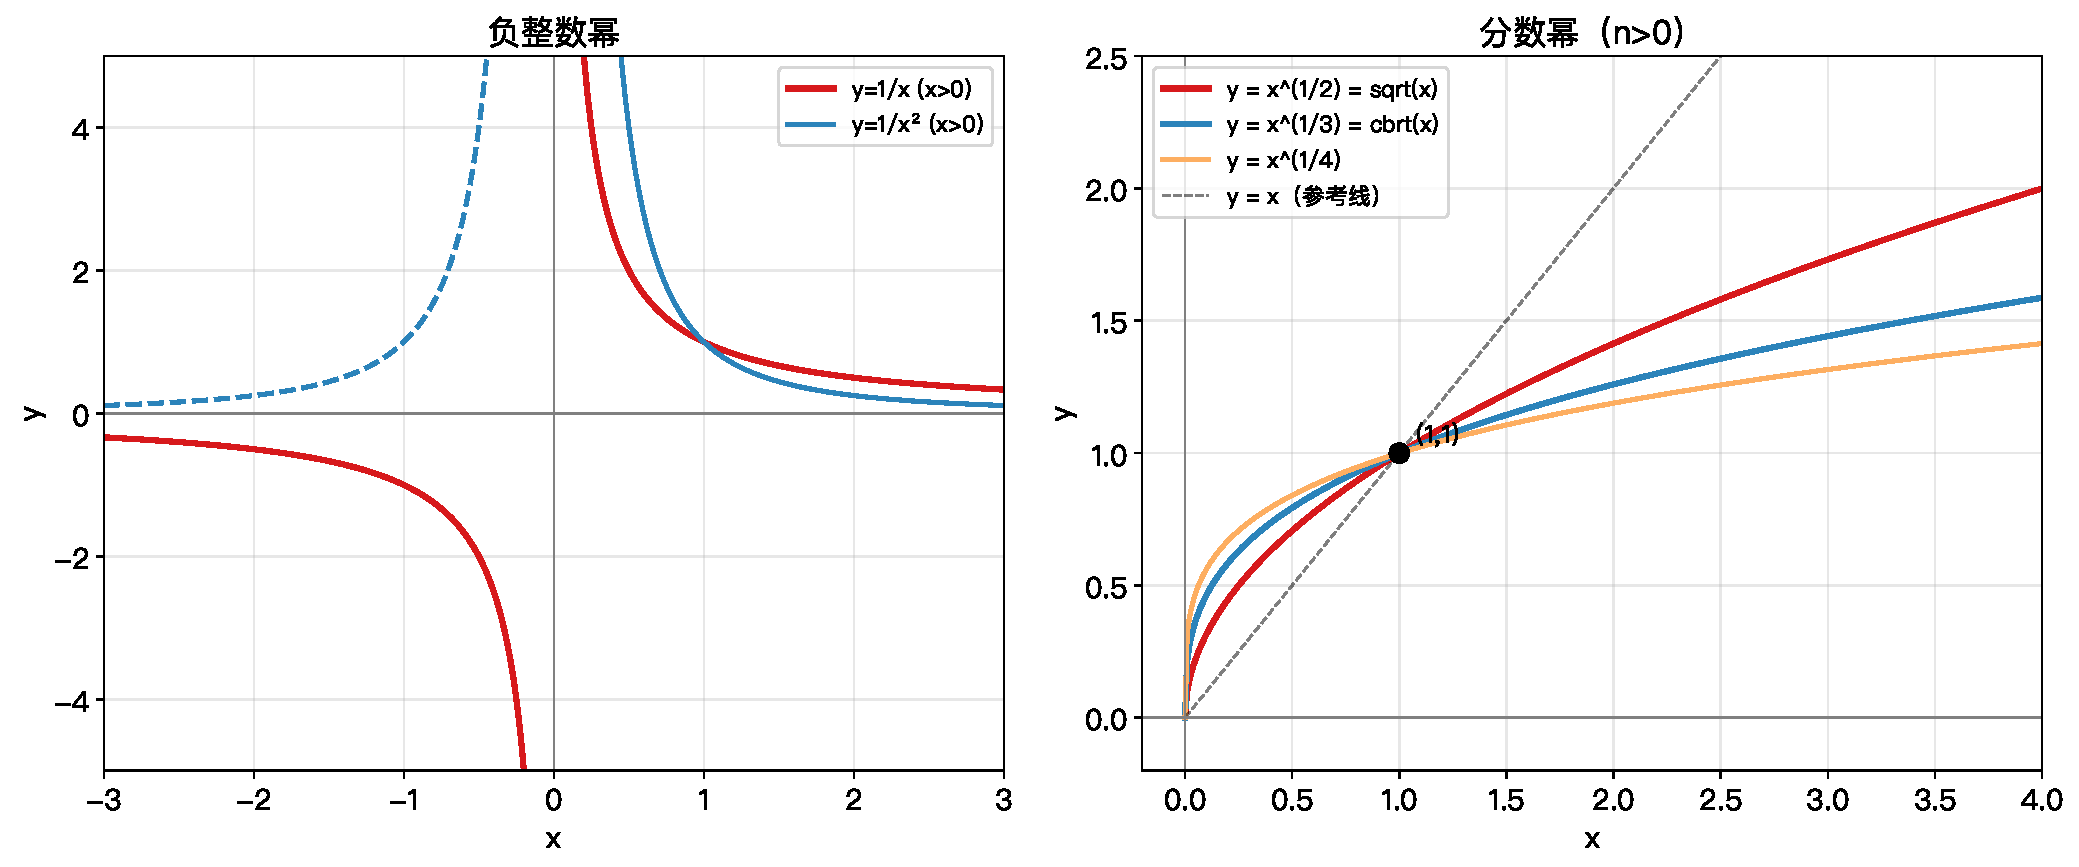
\includegraphics[width=0.55\textwidth]{figures/ch03_power_variants.pdf}
\end{center}

\textbf{关键区别：}
\begin{enumerate}
  \item 定义域：\(x \neq 0\)（分母不能为 0）
  \item \(y = 1/x\)（奇函数）：关于原点对称，图像穿过原点两侧
  \item \(y = 1/x^2\)（偶函数）：关于 \(y\) 轴对称，两侧都在 \(x\) 轴上方
  \item 当 \(x \to \pm\infty\) 时，\(y \to 0\)（水平渐近线 \(y = 0\)）
  \item 当 \(x \to 0\) 时，\(|y| \to \infty\)（垂直渐近线 \(x = 0\)）
\end{enumerate}
\end{examplebox}


% ============================================================
\section{分数幂——根号形式}
% ============================================================

当 \(n\) 是分数时，幂函数变成\textbf{根号形式}：
\[
x^{1/m} = \sqrt[m]{x}
\]

\begin{examplebox}[5]
对比 \(y = x^{1/2} = \sqrt{x}\)、\(y = x^{1/3}\)、\(y = x^{1/4}\)：

\begin{center}
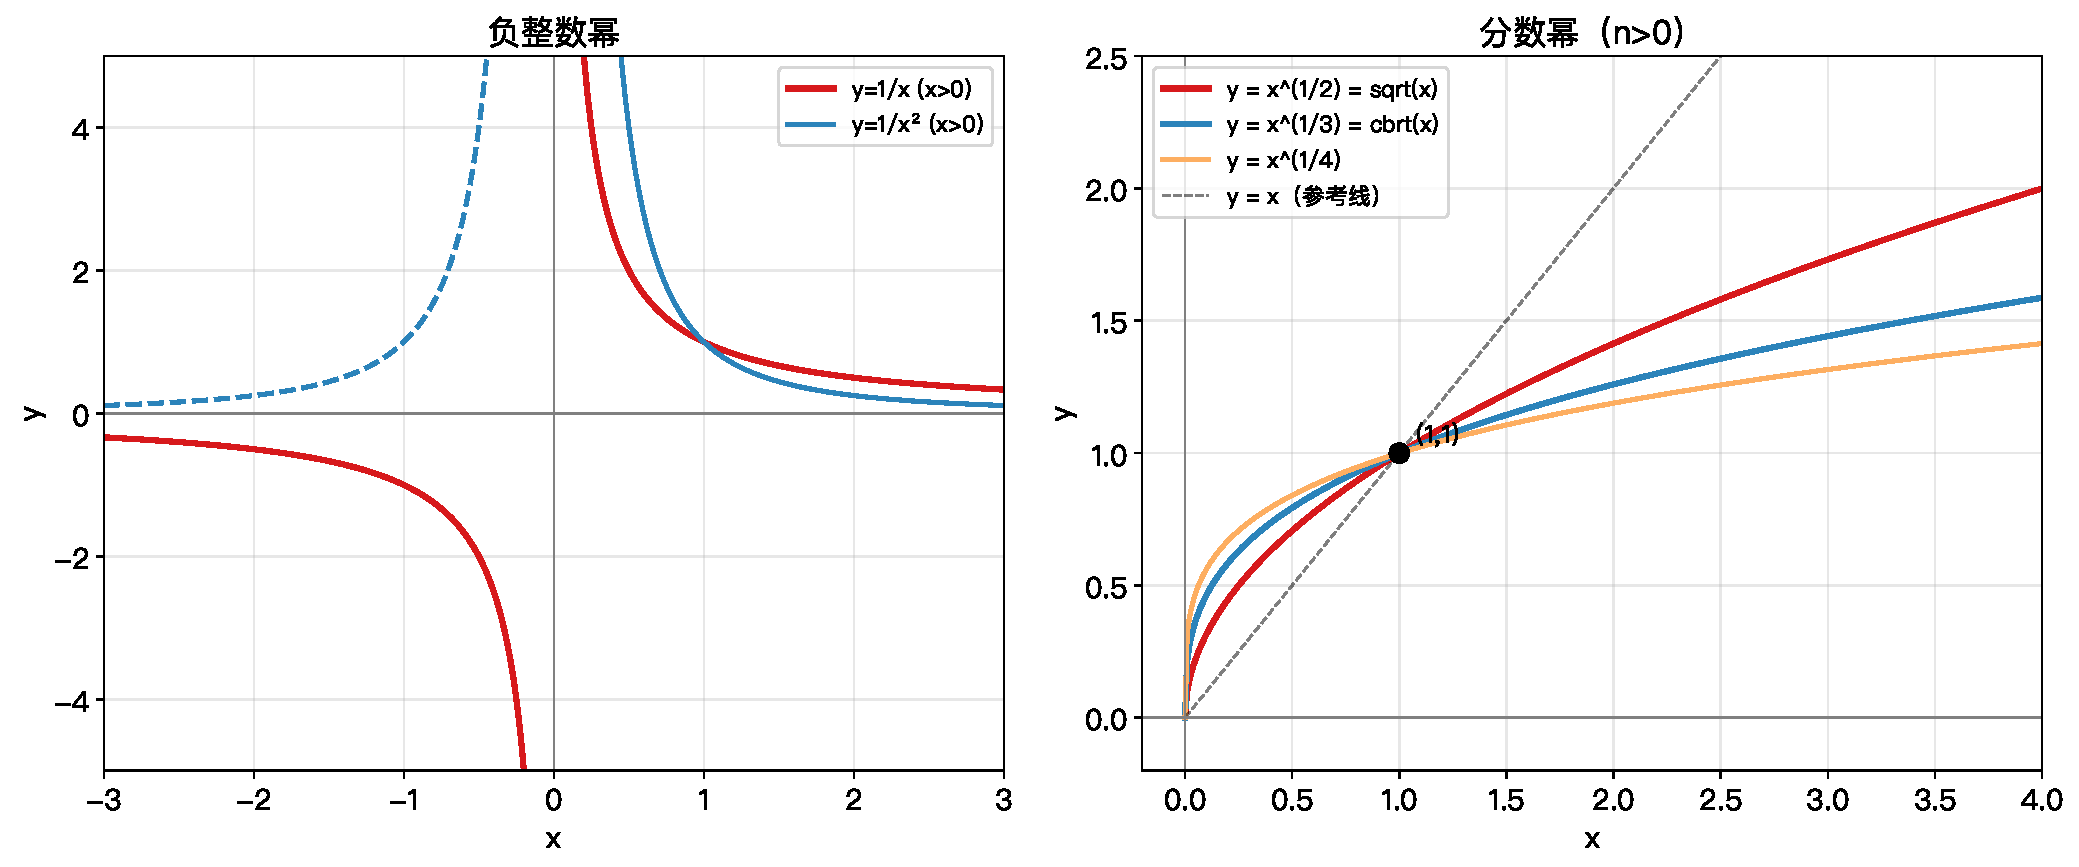
\includegraphics[width=0.55\textwidth]{figures/ch03_power_variants.pdf}
\end{center}

\textbf{规律：}
\begin{enumerate}
  \item 定义域：偶次根号（\(x^{1/2}, x^{1/4}\)）要求 \(x \ge 0\)；奇次根号（\(x^{1/3}\)）定义域为全体实数
  \item 所有分数幂都经过 \((0,0)\) 和 \((1,1)\)
  \item 在 \(x > 1\) 区域：指数越小，图像越靠近 \(x\) 轴（增长越慢）
  \item 分数幂的增长速度\textbf{慢于}直线 \(y = x\)——所以 \(\sqrt{x}\) 比 \(x\) 增长得慢
\end{enumerate}
\end{examplebox}


% ============================================================
\section{幂的运算规则}
% ============================================================

学习多项式之前，需要先巩固幂的运算。

\begin{definitionbox}[幂的运算法则]
设 \(a > 0\)，\(b > 0\)，\(m, n\) 为实数：
\begin{align*}
  a^m \cdot a^n &= a^{m+n} \quad &\text{（同底相乘，指数相加）} \\
  \frac{a^m}{a^n} &= a^{m-n} \quad &\text{（同底相除，指数相减）} \\
  (a^m)^n &= a^{mn} \quad &\text{（幂的乘方，指数相乘）} \\
  (ab)^n &= a^n \cdot b^n \quad &\text{（积的乘方，分别乘方）} \\
  a^{-n} &= \frac{1}{a^n} \quad &\text{（负指数 = 倒数）} \\
  a^{1/n} &= \sqrt[n]{a} \quad &\text{（分数指数 = 根号）}
\end{align*}
\end{definitionbox}

\begin{examplebox}[6——幂运算练习]
计算：
\[
(1)\; 2^3 \cdot 2^4 \qquad (2)\; \frac{3^5}{3^2} \qquad (3)\; (2^2)^3 \qquad (4)\; 8^{2/3}
\]

解：
\[
\begin{aligned}
(1)&\; 2^3 \cdot 2^4 = 2^{3+4} = 2^7 = 128 \\
(2)&\; \frac{3^5}{3^2} = 3^{5-2} = 3^3 = 27 \\
(3)&\; (2^2)^3 = 2^{2\times3} = 2^6 = 64 \\
(4)&\; 8^{2/3} = (8^{1/3})^2 = (\sqrt[3]{8})^2 = 2^2 = 4
\end{aligned}
\]
\end{examplebox}


% ============================================================
\section{多项式函数——幂函数的组合}
% ============================================================

把多个幂函数加起来，就得到了\textbf{多项式}。

\begin{definitionbox}[多项式函数]
形如
\[
P(x) = a_n x^n + a_{n-1} x^{n-1} + \cdots + a_1 x + a_0
\]
的函数称为\textbf{多项式函数}（读作 duō xiàng shì，英文 polynomial），
其中：
\begin{itemize}
  \item \(n\) 是\textbf{最高次数}（多项式的\textbf{次数}，degree）
  \item \(a_n\) 是\textbf{首项系数}（\(a_n \neq 0\)）
  \item \(a_0\) 是\textbf{常数项}
  \item 每一项 \(a_k x^k\) 是一个\textbf{单项式}
\end{itemize}
\end{definitionbox}

\begin{examplebox}[7——多项式举例]
\begin{align*}
  P(x) &= 3x^2 - 2x + 1 \quad &\text{二次多项式（首项系数 3，常数项 1）} \\
  Q(x) &= x^3 - 4x \quad &\text{三次多项式（缺 \(x^2\) 和常数项）} \\
  R(x) &= (x+1)(x-2)(x+3) \quad &\text{因式分解形式的三次多项式}
\end{align*}
\end{examplebox}


% ============================================================
\section{多项式的根——与 \(x\) 轴的交点}
% ============================================================

\begin{definitionbox}[多项式的根]
如果 \(P(r) = 0\)，则称 \(r\) 是多项式 \(P(x)\) 的\textbf{根}（读作 gēn，英文 root），
也叫\textbf{零点}（zero）。

几何意义：根就是函数图像与 \(x\) 轴交点的横坐标。
\end{definitionbox}

\begin{examplebox}[8]
多项式 \(f(x) = (x+2)(x-1)(x-3)\)：

\begin{center}
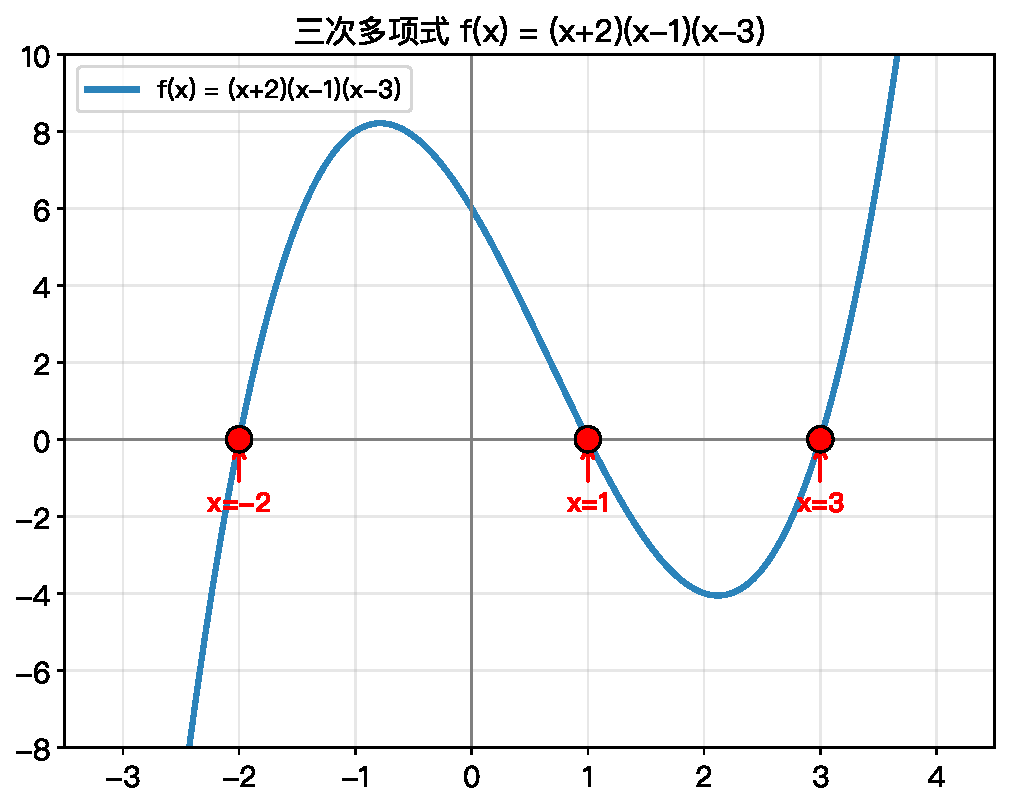
\includegraphics[width=0.6\textwidth]{figures/ch03_cubic_polynomial.pdf}
\end{center}

从图上一眼看出：
\begin{itemize}
  \item 根为 \(x = -2\)、\(x = 1\)、\(x = 3\)（三个根都是\textbf{单根}）
  \item 在根处，图像\textbf{穿过} \(x\) 轴（从一侧到另一侧）
  \item 三次多项式最多有 3 个根
\end{itemize}
\end{examplebox}

\begin{notebox}
多项式的\textbf{次数决定了最多有多少个根}：
\[
\text{\(n\) 次多项式最多有 \(n\) 个实数根}
\]
（可以有不到 \(n\) 个，因为有些根可能是复数——以后学。）
\end{notebox}


% ============================================================
\section{重根——图像"弹回"不穿过}
% ============================================================

如果多项式中某个因式出现了多次，这个根就叫做\textbf{重根}。

\begin{examplebox}[9]
对比单根和重根的行为：

\begin{center}
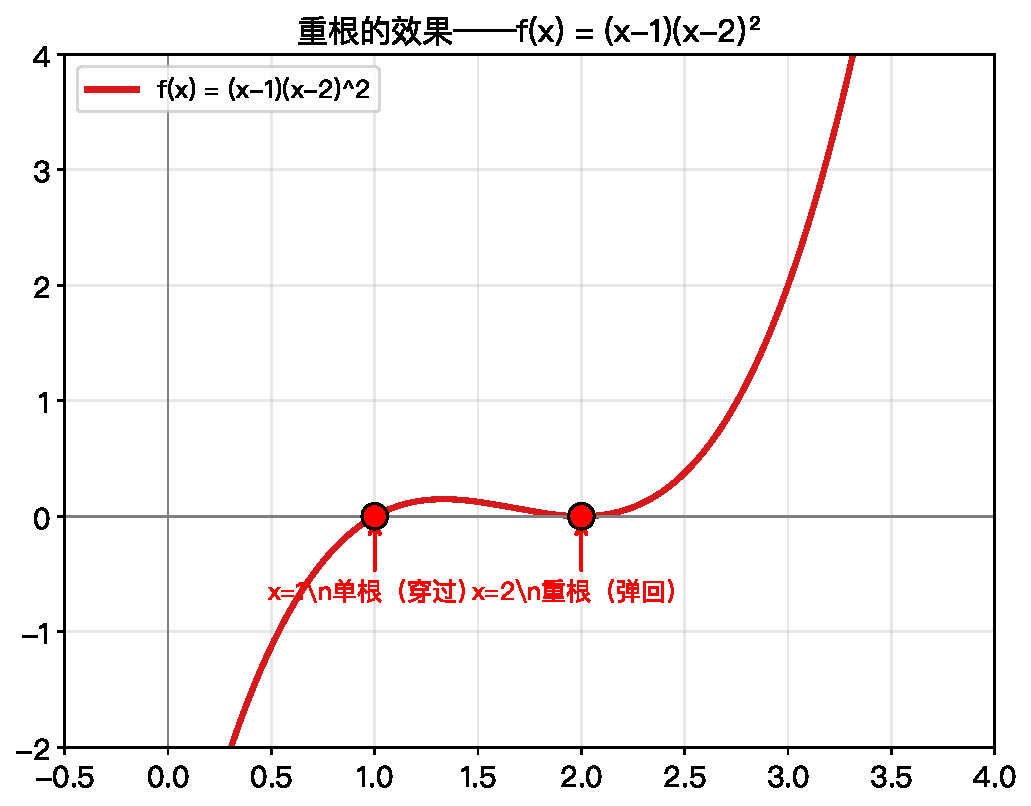
\includegraphics[width=0.6\textwidth]{figures/ch03_double_root.pdf}
\end{center}

\(f(x) = (x-1)(x-2)^2\)：
\begin{itemize}
  \item \(x = 1\)（单根）：图像\textbf{穿过} \(x\) 轴
  \item \(x = 2\)（二重根）：图像\textbf{碰到} \(x\) 轴然后\textbf{弹回}（不穿过）
\end{itemize}

\textbf{规律：}
\begin{center}
\begin{tabular}{c|c}
\textbf{重数} & \textbf{图像行为} \\
\hline
奇数次重根（单根、三重根等） & 穿过 \(x\) 轴 \\
偶数次重根（二重、四重根等） & 碰到 \(x\) 轴弹回 \\
\end{tabular}
\end{center}
\end{examplebox}


% ============================================================
\section{多项式的运算}
% ============================================================

\begin{examplebox}[10——多项式乘法]
展开 \((x+1)(x-2)(x+3)\)：

\[
\begin{aligned}
(x+1)(x-2)(x+3) &= (x^2 - 2x + x - 2)(x+3) \\
&= (x^2 - x - 2)(x+3) \\
&= x^3 + 3x^2 - x^2 - 3x - 2x - 6 \\
&= x^3 + 2x^2 - 5x - 6
\end{aligned}
\]

\textbf{验证：} 当 \(x = 1\) 时，原式 \((2)(-1)(4) = -8\)，展开式 \(1 + 2 - 5 - 6 = -8\) [OK]
\end{examplebox}

\begin{examplebox}[11——多项式除法（综合除法）]
用 \(x-2\) 除 \(x^3 + 2x^2 - 5x - 6\)：

\[
x^3 + 2x^2 - 5x - 6 = (x-2)(x^2 + 4x + 3)
\]

验证：\((x-2)(x^2 + 4x + 3) = x^3 + 4x^2 + 3x - 2x^2 - 8x - 6 = x^3 + 2x^2 - 5x - 6\) [OK]

所以 \(x=2\) 是多项式的一个根（\(f(2) = 8 + 8 - 10 - 6 = 0\)）。
\end{examplebox}

\begin{theorembox}[余数定理]
多项式 \(P(x)\) 除以 \((x-a)\) 的\textbf{余数}就是 \(P(a)\)。

特别地，如果 \(P(a) = 0\)，那么 \((x-a)\) 是 \(P(x)\) 的一个因式。
\end{theorembox}


% ============================================================
\section{符号卡片}
% ============================================================

\begin{symbolcard}
\(x^n\) & \verb|x^n| & 读作"x 的 n 次方" & 幂函数，底 \(x\) 指数 \(n\) \\
\(P(x)\) & \verb|P(x)| & 读作"P of x" & 多项式函数 \\
\(a_n x^n\) & \verb|a_n x^n| & —— & 多项式的第 \(n\) 次项 \\
\(r\) 是 \(P\) 的根 & \verb|P(r)=0| & 读作"P of r 等于 0" & \(r\) 使多项式值为 0 \\
重根 & —— & 读作"chóng gēn" & 因式出现多次的根 \\
\end{symbolcard}


% ============================================================
\section{代码验证}
% ============================================================

\begin{lstlisting}[caption=幂函数与多项式的数值验证]
import numpy as np

# 1. 验证幂函数经过 (1,1)
print("=== 所有幂函数都经过 (1,1) ===")
for n in [1, 2, 3, 4, -1, -2, 0.5]:
    print(f"  n={n:4.1f}:  1^{n} = {1**n}")

print()

# 2. 多项式的根
def f(x):
    return (x + 2) * (x - 1) * (x - 3)

print("=== 多项式的根 ===")
for test_x in [-2, 1, 3]:
    print(f"  f({test_x}) = {f(test_x)}  (应为0)")

print()

# 3. 奇函数性质验证：f(-x) = -f(x)
print("=== 奇函数验证 ===")
for x in [1, 2, 3.5]:
    lhs = x**3          # f(x) = x^3
    rhs_pos = x**3
    rhs_neg = (-x)**3
    print(f"  x={x:3.1f}:  ({x})^3 = {rhs_pos:6.1f},  ({-x})^3 = {rhs_neg:6.1f} = -{rhs_pos}")

print()

# 4. 偶函数验证：f(-x) = f(x)
print("=== 偶函数验证 ===")
for x in [1, 2, 3.5]:
    lhs = x**2
    rhs = (-x)**2
    print(f"  x={x:3.1f}:  ({x})^2 = {lhs:4.1f},  ({-x})^2 = {rhs:4.1f}  (相等)")
\end{lstlisting}

运行结果：
\begin{lstlisting}[frame=none,backgroundcolor={},numbers=none]
=== 所有幂函数都经过 (1,1) ===
  n= 1.0:  1^1 = 1
  n= 2.0:  1^2 = 1
  n= 3.0:  1^3 = 1
  n= 4.0:  1^4 = 1
  n=-1.0:  1^-1 = 1
  n=-2.0:  1^-2 = 1
  n= 0.5:  1^0.5 = 1

=== 多项式的根 ===
  f(-2) = 0  (应为0)
  f(1) = 0  (应为0)
  f(3) = 0  (应为0)

=== 奇函数验证 ===
  x=1.0:  (1)^3 =    1.0,  (-1)^3 =   -1.0 = -1.0
  x=2.0:  (2)^3 =    8.0,  (-2)^3 =   -8.0 = -8.0
  x=3.5:  (3.5)^3 =   42.9,  (-3.5)^3 =  -42.9 = -42.9

=== 偶函数验证 ===
  x=1.0:  (1)^2 = 1.0,  (-1)^2 = 1.0  (相等)
  x=2.0:  (2)^2 = 4.0,  (-2)^2 = 4.0  (相等)
  x=3.5:  (3.5)^2 = 12.2,  (-3.5)^2 = 12.2  (相等)
\end{lstlisting}


% ============================================================
\section{本章小结}
% ============================================================

\begin{progressbox}
\textbf{幂函数} \(y = x^n\)：底变、指数固定。所有幂函数经过 \((1,1)\)。

\textbf{指数 }\(n\) \textbf{决定行为}：
\begin{itemize}
  \item 正整数：\(n\) 越大增长越快，偶次幂"两头翘"，奇次幂"一低一高"
  \item 负整数：\(x^{-n} = 1/x^n\)，有渐近线 \(x=0\) 和 \(y=0\)
  \item 分数：\(x^{1/n} = \sqrt[n]{x}\)，增长慢于直线
\end{itemize}

\textbf{奇偶性}：\(f(-x) = f(x)\)（偶，关于 \(y\) 轴对称）
vs \(f(-x) = -f(x)\)（奇，关于原点对称）

\textbf{多项式}：幂函数的线性组合。\\
次数决定最多根数，重数的奇偶性决定图像是否穿过 \(x\) 轴。

\textbf{余数定理}：\(P(x)\) 除以 \((x-a)\) 的余数 = \(P(a)\)。
\end{progressbox}

\subsection*{通往下一章}

\textbf{这一章}你学会了幂函数和多项式——从简单的一次到高次的"弯曲"。

\textbf{下一章}我们进入\textbf{指数函数}——一种增长速度远超任何幂函数的函数。
为什么指数函数被称为"增长的终极武器"？为什么 AI 中的 Softmax 要用指数？下一章揭晓。


% ============================================================
% 习题
% ============================================================
\section{习题}

% ===== 送分 =====

\begin{exercise}[0]
判断是幂函数还是指数函数：
\[
(1)\; y = x^5 \qquad
(2)\; y = 5^x \qquad
(3)\; y = x^{1/3} \qquad
(4)\; y = 3^x
\]
\end{exercise}

\begin{exercise}[0]
计算：
\[
(1)\; 2^5 \qquad
(2)\; 3^{-2} \qquad
(3)\; 4^{1/2} \qquad
(4)\; 27^{1/3}
\]
\end{exercise}

\begin{exercise}[0]
判断奇偶性：\(y = x^4\) 是奇函数还是偶函数？\(y = x^5\) 呢？
\end{exercise}

\begin{exercise}[0]
多项式 \(f(x) = (x-1)(x-3)\) 的次数是几？它的根是什么？
\end{exercise}

% ===== 简单 =====

\begin{exercise}[1]
化简：
\[
(1)\; a^3 \cdot a^5 \qquad
(2)\; \frac{b^7}{b^4} \qquad
(3)\; (c^2)^4 \qquad
(4)\; (2x)^3
\]
\end{exercise}

\begin{exercise}[1]
画出 \(y = x^2\) 和 \(y = x^4\) 在同一坐标系中的草图（标出 \((1,1)\) 点）。
比较在 \(x=2\) 处哪个函数值更大。
\end{exercise}

\begin{exercise}[1]
多项式 \(f(x) = 2x^3 - 3x^2 + x - 5\)，求 \(f(0)\)、\(f(1)\)、\(f(-1)\)。
\end{exercise}

\begin{exercise}[1]
\(y = x^{-1}\) 和 \(y = x^{-2}\) 的定义域分别是什么？为什么？
\end{exercise}

% ===== 基础 =====

\begin{exercise}[2]
展开下列多项式：
\[
(1)\; (x+1)(x+2) \qquad
(2)\; (x-1)(x+3)(x-2) \qquad
(3)\; (x+2)^3
\]
\end{exercise}

\begin{exercise}[2]
求下列多项式的根：
\[
(1)\; f(x) = (x-4)(x+1) \qquad
(2)\; f(x) = (x-2)(x+3)(x-5)
\]
\end{exercise}

\begin{exercise}[2]
判断 \(x=2\) 是不是 \(f(x) = x^3 - 3x^2 + 4\) 的根（用余数定理）。
\end{exercise}

\begin{exercise}[2]
比较大小（不用计算器）：
\[
(1)\; 2^3 \text{ 和 } 3^2 \qquad
(2)\; 4^{1/2} \text{ 和 } 8^{1/3} \qquad
(3)\; 2^{-1} \text{ 和 } 3^{-1}
\]
\end{exercise}

% ===== 普通 =====

\begin{exercise}[3]
多项式 \(f(x) = x^3 - 2x^2 - 5x + 6\) 的一个根是 \(x=1\)。
\begin{enumerate}
  \item[(1)] 用多项式除法求另外两个根
  \item[(2)] 写出 \(f(x)\) 的因式分解形式
\end{enumerate}
\end{exercise}

\begin{exercise}[3]
已知 \(f(x) = (x+1)(x-2)^2\)。
\begin{enumerate}
  \item[(1)] 展开为一般形式
  \item[(2)] 指出每个根的重数
  \item[(3)] 在根 \(x=2\) 处，图像穿过还是弹回？
\end{enumerate}
\end{exercise}

\begin{exercise}[3]
画出下列函数的草图（利用幂函数图像平移得到）：
\[
(1)\; y = (x-1)^3 \qquad
(2)\; y = x^2 + 2
\]
\end{exercise}

\begin{exercise}[3]
证明 \(x=3\) 是 \(f(x) = x^4 - 3x^3 - 3x^2 + 11x - 6\) 的根，
然后用除法分解出 \((x-3)\)。
\end{exercise}

\begin{exercise}[3]
一个矩形的长比宽多 2 米，面积是 15 平方米。设宽为 \(x\) 米：
\begin{enumerate}
  \item[(1)] 列出关于 \(x\) 的二次方程
  \item[(2)] 解出 \(x\)（根），取有实际意义的值
\end{enumerate}
\end{exercise}

\begin{exercise}[3]
判断正误并说明理由：
\[
y = x^2 \text{ 和 } y = x^4 \text{ 在 } x < -1 \text{ 时，} x^4 > x^2 > 0
\]
\end{exercise}

% ===== 中等 =====

\begin{exercise}[4]
多项式 \(f(x) = x^4 - 5x^2 + 4\)。
\begin{enumerate}
  \item[(1)] 令 \(t = x^2\)，将 \(f(x)\) 化为关于 \(t\) 的二次方程
  \item[(2)] 解出所有的根
\end{enumerate}
\end{exercise}

\begin{exercise}[4]
已知 \(f(x) = x^3 + ax^2 + bx + c\) 的根是 \(-2\)、\(1\)、\(3\)，求 \(a\)、\(b\)、\(c\)。
\end{exercise}

\begin{exercise}[4]
比较 \(y = x^{10}\) 和 \(y = 10^x\)：当 \(x=2\) 时哪个大？当 \(x=10\) 时呢？
从这个比较中你能得出什么结论？
\end{exercise}

\begin{exercise}[4]
三次多项式 \(f(x)\) 在 \(x=-1\) 处有单根，在 \(x=2\) 处有二重根，且 \(f(0)=4\)，求 \(f(x)\) 的表达式。
\end{exercise}

\begin{exercise}[4]
已知函数的图像经过以下变换，写出新函数表达式：
\[
y = x^3 \xrightarrow{\text{右移 1}} \xrightarrow{\text{上移 2}} \xrightarrow{\text{关于 x 轴对称}}
\]
\end{exercise}

% ===== 进阶 =====

\begin{exercise}[5]
多项式 \(f(x) = 2x^4 - 3x^3 + 2x - 1\) 除以 \(x-2\)，求余数（用余数定理，不要做除法）。
\end{exercise}

\begin{exercise}[5]
\(f(x) = x^4 - 2x^2 + 1\) 有几个根？哪些是重根？
（提示：先因式分解 \(x^4 - 2x^2 + 1\)）
\end{exercise}

\begin{exercise}[5]
对于多项式 \(f(x) = (x^2 - 1)(x^2 - 4)\)：
\begin{enumerate}
  \item[(1)] 展开
  \item[(2)] 求所有根
  \item[(3)] 描述图像在每一个根处的行为（穿过还是弹回）
\end{enumerate}
\end{exercise}

% ===== 拔高 =====

\begin{exercise}[6]
已知 \(f(x) = x^3 - 3x^2 + 2\)。
\begin{enumerate}
  \item[(1)] 验证 \(x=1\) 是一个根
  \item[(2)] 做多项式除法，将 \(f(x)\) 因式分解
  \item[(3)] 画出 \(f(x)\) 的草图（标出根和关键点的坐标）
  \item[(4)] 解不等式 \(f(x) > 0\)
\end{enumerate}
\end{exercise}

\begin{exercise}[6]
多项式 \(P(x) = 2x^4 - 9x^3 + 12x^2 - 4x\)。
\begin{enumerate}
  \item[(1)] 提公因式 \(x\)，得到一个根
  \item[(2)] 对剩下的三次多项式猜根（尝试 \(x=1,2\)），做除法
  \item[(3)] 写出 \(P(x)\) 的完全因式分解
  \item[(4)] \(x=2\) 是几重根？
\end{enumerate}
\end{exercise}

\begin{exercise}[6]
证明：两个奇函数的乘积是偶函数；一个奇函数和一个偶函数的乘积是奇函数。
（提示：设 \(f\) 奇、\(g\) 奇，检查 \(f(-x)g(-x)\) 等于什么）
\end{exercise}

% ===== 极难 =====

\begin{exercise}[7]
已知多项式 \(P(x) = x^3 + ax^2 + bx + c\) 满足：
\[
P(1) = 0,\quad P(2) = 0,\quad P(3) = 6
\]
\begin{enumerate}
  \item[(1)] 利用前两个条件，设 \(P(x) = (x-1)(x-2)(x+k)\)，求 \(k\)
  \item[(2)] 用第三个条件解出 \(k\)，展开求 \(a,b,c\)
  \item[(3)] 验证 \(P(0)\) 的值
\end{enumerate}

\textbf{说明：} 这道题综合了根、因式分解、待定系数法三个知识点。
多项式的待定系数法是数学分析中常用的技巧。
\end{exercise}
